% Généré par md2tex.py — ne pas éditer à la main ; éditer le .md maître et reconvertir.
% Compile : pdflatex (deux fois si besoin).
\documentclass[11pt]{article}
\usepackage[T1]{fontenc}
\usepackage[utf8]{inputenc}
\usepackage{lmodern}
\usepackage{textcomp}
\usepackage[margin=1in]{geometry}
\usepackage{booktabs,array}
\usepackage{amsmath,amssymb}
\usepackage{graphicx}
\usepackage{caption}
\usepackage{adjustbox}
\usepackage{enumitem}
\usepackage[hidelinks]{hyperref}
\usepackage{newunicodechar}
\newunicodechar{·}{\ensuremath{\cdot}}
\newunicodechar{×}{\ensuremath{\times}}
\newunicodechar{÷}{\ensuremath{\div}}
\newunicodechar{¬}{\ensuremath{\neg}}
\newunicodechar{µ}{\ensuremath{\mu}}
\newunicodechar{²}{\textsuperscript{2}}
\newunicodechar{ᵉ}{\textsuperscript{e}}
\newunicodechar{′}{\ensuremath{'}}
\newunicodechar{Δ}{\ensuremath{\Delta}}
\newunicodechar{α}{\ensuremath{\alpha}}
\newunicodechar{β}{\ensuremath{\beta}}
\newunicodechar{δ}{\ensuremath{\delta}}
\newunicodechar{ε}{\ensuremath{\varepsilon}}
\newunicodechar{η}{\ensuremath{\eta}}
\newunicodechar{ρ}{\ensuremath{\rho}}
\newunicodechar{←}{\ensuremath{\leftarrow}}
\newunicodechar{→}{\ensuremath{\rightarrow}}
\newunicodechar{↔}{\ensuremath{\leftrightarrow}}
\newunicodechar{⇒}{\ensuremath{\Rightarrow}}
\newunicodechar{⟹}{\ensuremath{\Longrightarrow}}
\newunicodechar{∈}{\ensuremath{\in}}
\newunicodechar{−}{\ensuremath{-}}
\newunicodechar{∖}{\ensuremath{\setminus}}
\newunicodechar{∝}{\ensuremath{\propto}}
\newunicodechar{∧}{\ensuremath{\wedge}}
\newunicodechar{∪}{\ensuremath{\cup}}
\newunicodechar{≈}{\ensuremath{\approx}}
\newunicodechar{≡}{\ensuremath{\equiv}}
\newunicodechar{≤}{\ensuremath{\leq}}
\newunicodechar{≥}{\ensuremath{\geq}}
\newunicodechar{⊆}{\ensuremath{\subseteq}}
\newunicodechar{⊑}{\ensuremath{\sqsubseteq}}
\newunicodechar{⊘}{\ensuremath{\oslash}}
\newunicodechar{⊨}{\ensuremath{\models}}
\newunicodechar{▲}{\ensuremath{\blacktriangle}}
\newunicodechar{◇}{\ensuremath{\Diamond}}
\newunicodechar{✓}{\checkmark}
\newunicodechar{✕}{\ensuremath{\times}}
\setlist{nosep,leftmargin=1.5em}
\setlength{\parskip}{4pt}\setlength{\parindent}{0pt}
\renewcommand{\abstractname}{Résumé}
\title{\textbf{Apprentissage de bibliothèque défaisable : des méthodes typées à contrats d'exécution qui se désapprennent à la dérive}}
\author{Nathanael Braun · skynet-graph · 2026-06-29}
\date{2026}
\begin{document}
\maketitle
\begin{quote}\itshape \textbf{v2 — 2026-07-04.} Révision éditoriale de la version déposée (Zenodo) : structure didactique des paragraphes, terminologie alignée sur le canon \texttt{concept-*} du moteur hôte, référence croisée vers l'article compagnon sur la porte d'admission [Braun 2026b], et sept figures F1–F7 générées depuis les harnais déterministes de l'artefact. \textbf{Les expériences, les chiffres et les revendications sont ceux de la v1 déposée, inchangés.}\end{quote}

\medskip\hrule\medskip

\section*{Résumé}

Les agents LLM réutilisent leur travail passé via une mémoire \emph{floue} : la recherche documentaire (RAG), le raisonnement à partir de cas (CBR), ou encore les bibliothèques de compétences en prose. Toutes ces mémoires rappellent par similarité de surface — la ressemblance entre la requête et l'entrée stockée, jamais la validité de ce qui la justifie ; aucune, donc, ne sait représenter une \emph{prémisse devenue fausse} — ce que nous appelons la \textbf{dérive} : le monde change (une réglementation se durcit, un fait est audité et trouvé faux) sans que la requête change. La réponse en cache reste alors le plus proche voisin, et elle est servie quand même. Les bibliothèques apprises statiques ont le défaut inverse : elles sont saines une fois apprises, mais incapables de \emph{désapprendre}.

Nous présentons l'\textbf{apprentissage de bibliothèque défaisable}. L'objet est une bibliothèque apprise de \textbf{méthodes} — des unités de travail réutilisables dont les entrées, les sorties et les conditions sont des faits typés — chacune portant un \textbf{contrat d'exécution défaisable} : ce qu'elle lit, ce qu'elle écrit, ce qu'elle exige et ce qu'elle garantit. Le mécanisme tient en une boucle : la garantie d'une méthode est \emph{supposée} à sa composition, \emph{vérifiée} à son exécution, et \textbf{rétractée avec blâme} quand la vérification échoue — une étape de maintien de la vérité, au sens des TMS — après quoi la bibliothèque est \emph{révisée} chirurgicalement, non jetée. La même structure typée qui rend une méthode canonicalisable rend aussi sa réutilisation \emph{amortissable} (les cas récurrents éludent l'appel modèle) et sa composition \emph{vérifiable sur les seuls contrats}, à contexte par appel borné. Aucun mécanisme n'est nouveau en soi (JTMS, contrats-à-blâme, apprentissage de bibliothèque, empreintes à la logique de séparation) ; la contribution est leur \textbf{composition} en une représentation unique où amortissement, vérification de composition et \emph{désapprentissage principiel et sélectif à la dérive} coïncident — ce qu'aucune des briques ne fournit seule.

Nous évaluons chaque mécanisme isolément sur un moteur réel à base de règles — d'abord sous un simulateur déterministe, puis avec un modèle local en réel. Sous une dérive externe en cours de flux, les mémoires par rappel seul servent du \emph{périmé}, tandis que le contrat déclaratif récupère l'exactitude \emph{sélectivement} et \emph{en sûreté de composition} — pour une méthode seule, à travers une chaîne de méthodes apprise, et en tête-à-tête face aux systèmes de mémoire d'agents nommés (MemGPT, Reflexion, GraphRAG). Le tout est borné par un plafond honnête, mesuré, que nous appelons \textbf{K1} : seule la fraction typée et canonicalisable de la charge amortit.

\medskip\hrule\medskip

\section*{1. Introduction}

Un agent qui résout de nombreux problèmes apparentés devrait devenir moins coûteux et plus fiable avec le temps. La voie dominante aujourd'hui consiste à mémoriser et rappeler : stocker des solutions ou compétences passées, retrouver la plus proche pour un nouveau cas, la réutiliser ou l'adapter. La génération augmentée par recherche [Lewis et al. 2020], le raisonnement à partir de cas et les bibliothèques de compétences en prose comme Voyager [Wang et al. 2023] partagent cette forme — et le même angle mort : tous trois rappellent par similarité de \emph{surface} et ne représentent pas une \emph{prémisse devenue fausse}. Quand le monde change d'une manière qui ne change \textbf{pas} la requête — une réglementation se durcit, un fait est audité et trouvé faux, une politique est révoquée — la réponse en cache reste le plus proche voisin, et elle est toujours servie.

La mémoire est périmée avec assurance.

Les bibliothèques statiques (programmes appris, macro-opérateurs, compétences distillées [Ellis et al. 2021; Bowers et al. 2023]) ont le problème inverse : saines à l'apprentissage, elles ne savent pas \emph{désapprendre}. Aucun mécanisme ne fait en sorte que l'arrivée d'un fait contradictoire rétracte une réutilisation auparavant justifiée.

Nous soutenons que l'ingrédient manquant est un \textbf{contrat typé défaisable} attaché à chaque unité réutilisable. Empruntant aux contrats logiciels avec blâme [Findler \& Felleisen 2002] et à la vérification graduelle [Bader, Aldrich \& Tanter 2018], une méthode déclare ce qu'elle lit, ce qu'elle écrit, ce qu'elle exige et ce qu'elle garantit — sur un alphabet de faits \emph{typé}. La garantie d'une méthode \emph{apprise} est une hypothèse induite : elle est donc \textbf{supposée} à la composition, \textbf{vérifiée} à l'exécution et \textbf{rétractée avec blâme} en cas de violation. La rétractation est une opération de maintien de la vérité [Doyle 1979; de Kleer 1986] : la clôture de dépendance de la prémisse falsifiée s'effondre et aucune croyance fausse n'est servie ; la bibliothèque est ensuite révisée en \emph{spécialisant} la précondition fautive, non en supprimant la méthode.

La même structure typée procure, au-delà du désapprentissage, deux propriétés de plus. D'abord, la réutilisation \textbf{amortit} : une méthode dont l'applicabilité et les effets sont entièrement typés a une clé canonique stable, donc les cas récurrents éludent l'appel au modèle. Ensuite, la composition est \textbf{vérifiable sans ouvrir la boîte} : deux méthodes se composent sainement si et seulement si, sur les clés typées que l'une écrit et l'autre lit, la postcondition de la première implique la précondition de la seconde — une vérification décidable sur un alphabet fini [O'Hearn, Reynolds \& Yang 2001; Reynolds 2002] qui permet à un superviseur de porter des \emph{contrats}, pas des corps, gardant le contexte par appel borné.

Cette puissance est bornée par une unique contrainte honnête que nous appelons \textbf{K1} : seule la structure typée, canonicalisable, amortit ; un composant de décision véritablement en prose reste dans le modèle. Nous en mesurons la conséquence plutôt que de la masquer.

Nous employons \emph{apprentissage de bibliothèque} au sens établi de DreamCoder et Stitch [Ellis et al. 2021; Bowers et al. 2023] — induire des méthodes typées réutilisables à partir de traces par abstraction — non au sens d'un ajustement statistique de paramètres ; on pourrait tout aussi bien parler d'\emph{induction de méthodes}. La nouveauté ici n'est \textbf{aucun} mécanisme isolé — ni l'induction ni la maintenance de la vérité, toutes deux relevant d'un état de l'art vieux de plusieurs décennies — mais leur \textbf{composition} : attacher un contrat défaisable à une méthode \emph{typée et composable}, c'est ce qui fait découler l'amortissement, la vérification de composition et le désapprentissage d'une seule et même représentation, là où chaque brique seule ne livre au plus qu'un de ces trois bénéfices. Le changement est de l'ordre du flot de contrôle : là où une mémoire par similarité fait \texttt{requête → retrouver → réutiliser}, la nôtre fait \texttt{requête → retrouver-le-contrat → vérifier → exécuter → contrôler → rétracter → spécialiser}.

Le suffixe contrôler-et-rétracter — absent de la recherche, du CBR et des bibliothèques de compétences — fait toute la différence, et c'est lui que les expériences isolent.

\textbf{Contributions.} (1) Le cadrage des méthodes d'agent réutilisables comme \textbf{non-terminaux typés à deux faces} — boîte noire contractuelle pour l'appelant, productions typées à l'intérieur (§2.1) — \textbf{dotés d'un contrat d'exécution défaisable}, et la boucle supposer / vérifier / rétracter-blâmer / réviser qui se désapprend à la dérive. (2) Une évaluation reproductible, isolant les mécanismes, sur un moteur réel — la mémoire par rappel seul ne peut pas désapprendre tandis qu'un contrat typé déclaratif récupère la dérive \emph{sélectivement, généralement, sûrement-en-composition} (E2, simu + réel, avec une référence Invalidant équitable) ; transfert structurel sain que le seul nombre d'appels ne certifie pas (E1) ; aucun faux-admis sur les compositions évaluées, chacune des trois barrières ablée (E3) ; amortissement en gradient de la fraction canonicalisable (P4). Nous explicitons ce que chaque expérience établit ou non (petit n, simulateur déterministe, modèle réel unique).

\medskip\hrule\medskip

\section*{2. Approche}

L'approche se construit en trois questions, dans l'ordre où elles se posent : quel est l'objet réutilisable (§2.1) ; quel contrat cet objet doit-il porter pour que sa réutilisation soit sûre (§2.2) ; et dans quel pipeline cet objet vit-il, avec quel filet quand il manque (§2.3). Chaque réponse rend la suivante possible.

\subsection*{2.1 L'objet : une méthode à deux faces}

Première question : quel est l'objet réutilisable ? Une \textbf{méthode} est, pour son appelant, une boîte noire unique dotée d'un contrat typé ; à l'intérieur, une ou plusieurs \emph{productions} — les pas élémentaires (séquence, branchement, map, fold) — la réalisent. Dans la nomenclature du moteur hôte, c'est une \emph{concept-méthode} : l'unité apprise, à côté des \emph{concept-règles} autorées et des \emph{concept-sortes} du treillis de types. Formellement, c'est un non-terminal de remplacement d'hyperarêtes [Habel 1992; Drewes, Kreowski \& Habel 1997] à sélection conditionnée par précondition [Erol, Hendler \& Nau 1994]. Nous tenons deux régimes séparés par \emph{intention de conception} (nous ne prouvons pas la décidabilité ici). La \textbf{grammaire des méthodes} — sélection, paramétrage, composition — est \emph{censée} rester décidable, via un rang de montage bien fondé et un petit ensemble d'invariants de typage ; comme l'existence d'un plan HTN récursif est indécidable en général [Erol, Hendler \& Nau 1996], nous restreignons délibérément au fragment bien fondé. L'\textbf{exécution}, elle — le passage des données réelles à travers la méthode —, est le régime inverse : une couche explicitement bornée par un budget (« carburant »), Turing-complète. Le lien à la définissabilité en logique monadique du second ordre [Courcelle 1990] est offert comme motivation de la \emph{traitabilité possible} des vérifications grammaticales, non comme un théorème établi ici ; une preuve de décidabilité est laissée en travaux futurs.

\subsection*{2.2 Le contrat : un triplet de séparation défaisable}

L'objet est posé ; la question devient : quel contrat doit-il porter pour que sa réutilisation soit sûre ? Une méthode déclare une \textbf{empreinte de lecture} et une \textbf{empreinte d'écriture} (une \emph{empreinte} est l'ensemble des clés typées que la méthode touche), une \textbf{précondition} sur ce qu'elle lit, une \textbf{postcondition} sur ce qu'elle écrit et une \textbf{étiquette d'effet} (pure, ou porteuse d'un effet externe à vérifier). La composition sous état partagé est le problème du cadre [McCarthy \& Hayes 1969] ; nous le levons par une discipline d'empreintes issue de la logique de séparation [O'Hearn, Reynolds \& Yang 2001; Reynolds 2002] sur l'alphabet typé fini — le régime traitable, sans aliasing. Pour une méthode \emph{apprise} la postcondition est une hypothèse induite : \textbf{supposée à la composition, vérifiée à la stabilisation (le point fixe d'exécution du moteur), rétractée avec blâme en cas de violation} [Findler \& Felleisen 2002; Bader, Aldrich \& Tanter 2018]. Le moniteur d'exécution est le JTMS [Doyle 1979], et le résultat est une sûreté \emph{éventuelle} (non statique) — précisément le désapprentissage qui manque aux références floues. Ce désapprentissage est symbolique (une rétractation de croyance par JTMS) et distinct du \emph{machine unlearning} paramétrique [Bourtoule et al. 2021], qui efface l'influence de données d'entraînement des poids d'un modèle.

\begin{figure}[htbp]\centering
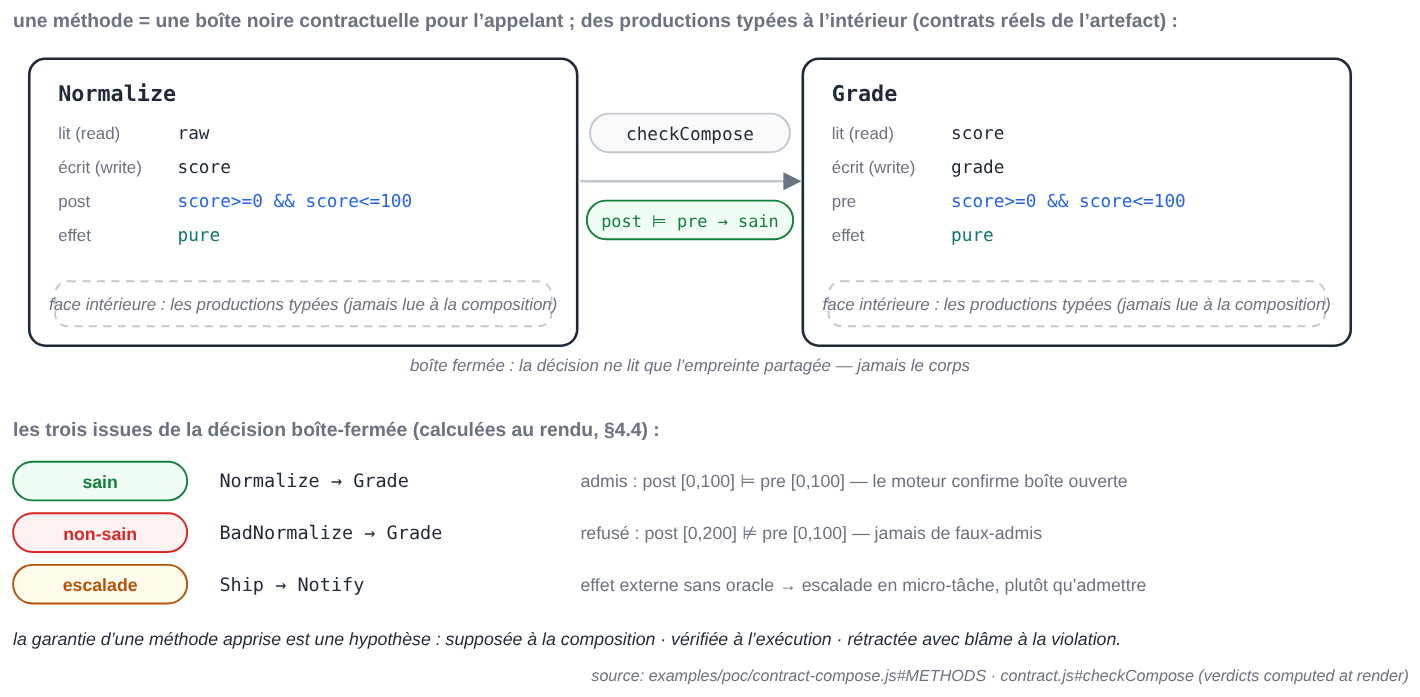
\includegraphics[width=\linewidth]{../figures/png/f1-method-contract.fr.png}
\caption*{\small Figure F1 — la méthode à deux faces : pour l'appelant, une boîte noire contractuelle (empreintes lit/écrit, pre/post, étiquette d'effet — les contrats réels de l'artefact) ; à l'intérieur, les productions typées, jamais lues à la composition. Entre deux méthodes, la décision boîte-fermée \texttt{checkCompose} a trois issues — sain / non-sain / escalade —, calculées au rendu de la figure (§4.4).}
\end{figure}

\subsection*{2.3 Le pipeline et le plancher K1}

Reste la troisième question : dans quel pipeline cette méthode vit-elle, et avec quel filet quand elle manque ? Le pipeline, de bout en bout : une formulation humaine est typée en un but ; une méthode est sélectionnée et composée sur ses contrats ; les cas la traversent ; les traces se distillent en de nouvelles méthodes typées (anti-unification [Plotkin 1970], filtrée par MDL comme dans DreamCoder/Stitch [Ellis et al. 2021; Bowers et al. 2023]) ; et la dérive rétracte ce qu'elle invalide. L'étape d'\emph{admission} de ce pipeline — sous quelles conditions une unité apprise depuis un épisode LLM bruité a le droit d'entrer dans la bibliothèque — est l'objet de l'article compagnon [Braun 2026b], qui fournit la porte d'admission à attribution localisée (restriction de slot, arête de treillis, alias de surface) que la boucle décrite ici suppose en amont.

Le repli universel est le \textbf{plancher de micro-tâches} : tout ce qui ne se réduit pas à une méthode typée en cache se réduit à une micro-tâche qu'un petit modèle traite aisément.

Ainsi un contrat \emph{manquant} coûte un appel modèle bon marché (un gradient de coût gracieux), et un contrat \emph{faux} est rattrapé par la vérification d'exécution — les deux modes de défaillance dégradent respectivement le coût et déclenchent le désapprentissage, jamais une erreur silencieuse.

\medskip\hrule\medskip

\section*{3. Mise en œuvre}

Tous les mécanismes sont réalisés sur un moteur existant de graphe de faits typés à base de règles, cohérent par JTMS, à concepts déclaratifs et stabilisation par chaînage avant, sans modification de son cœur hormis une option de requête additive et rétrocompatible. La clé de mémoïsation typée est le condensé de canonicalisation du moteur ; le vérificateur de contrat défaisable (implication à la composition sur domaines abstraits, une assertion de postcondition à l'exécution, et trois barrières de sûreté) et la transformation de transfert structurel (relativiser-au-stockage / lier-au-rejeu) sont des bibliothèques hôtes au-dessus du moteur. Un exécuteur de cas qui fait tourner les méthodes validées de façon durable à l'échelle est un artefact d'ingénierie connu (un réseau de workflow [van der Aalst 1998] sur un magasin durable, dans la lignée d'AWS Step Functions Distributed Map [AWS 2022], du cache de contenu de Prefect, et de DBOS [Skiadopoulos et al. 2021]) ; notre \textbf{vue-croyance} — le graphe de croyances typées maintenu par le JTMS, par opposition à cette couche d'exécution durable — se situe au-dessus.

Le cycle de vie défaisable — \textbf{supposer → vérifier → contrôler → rétracter → spécialiser} — est tout le mécanisme, en correspondance un-à-un avec les fonctions du moteur qu'il appelle :

\begin{small}\begin{verbatim}
select(but):                                    # SUPPOSER (à la composition)
    M ← bibliothèque.match(but.faits_typés)     #   clé typée ; un échec retombe au plancher de micro-tâches
    supposer M.contrat                          #   checkCompose : post(préc.) ⊨ pre(M) ; escalade, jamais faux-admis

apply(M, cas):                                  # VÉRIFIER + CONTRÔLER (à l'exécution)
    clé ← digest(cas.prémisse_typée)            #   clé canonique K1
    si memo.has(clé) : retourner memo[clé]      #   amortir un cas typé récurrent
    sortie ← run(M, cas)                        #   sinon dériver (appel modèle / sous-graphe)
    si non assertPost(M.contrat, sortie) :      #   la post tient ? + G1 complétude-de-cadre + G2 oracle-d'effet
        quarantaine(cas) ; blâmer(M.contrat)    #   ne jamais valider une mauvaise sortie
        retourner
    memo[clé] ← sortie ; retourner sortie

on ingest(fait):                                # RÉTRACTER + SPÉCIALISER (dérive)
    pour e dans memo t.q. e dépend de fait :     #   JTMS : re-vérifier chaque post affectée face au nouveau fait
        si non satisfies(e.contrat.post, e.faits ∪ {fait}) :
            rétracter(e) ; blâmer(e.contrat)     #   désapprendre : évincer l'entrée invalidée + attribuer le blâme
    bibliothèque.réviser(blâme) : pre ← spécialiser(pre)  #   reviseOnBlame (CEGIS, synthèse guidée par contre-exemples) : restreindre la pre, sans supprimer
\end{verbatim}\end{small}

Le suffixe contrôler-et-rétracter est la seule partie absente d'une mémoire par similarité, et c'est exactement celle que les expériences isolent.

\begin{figure}[htbp]\centering
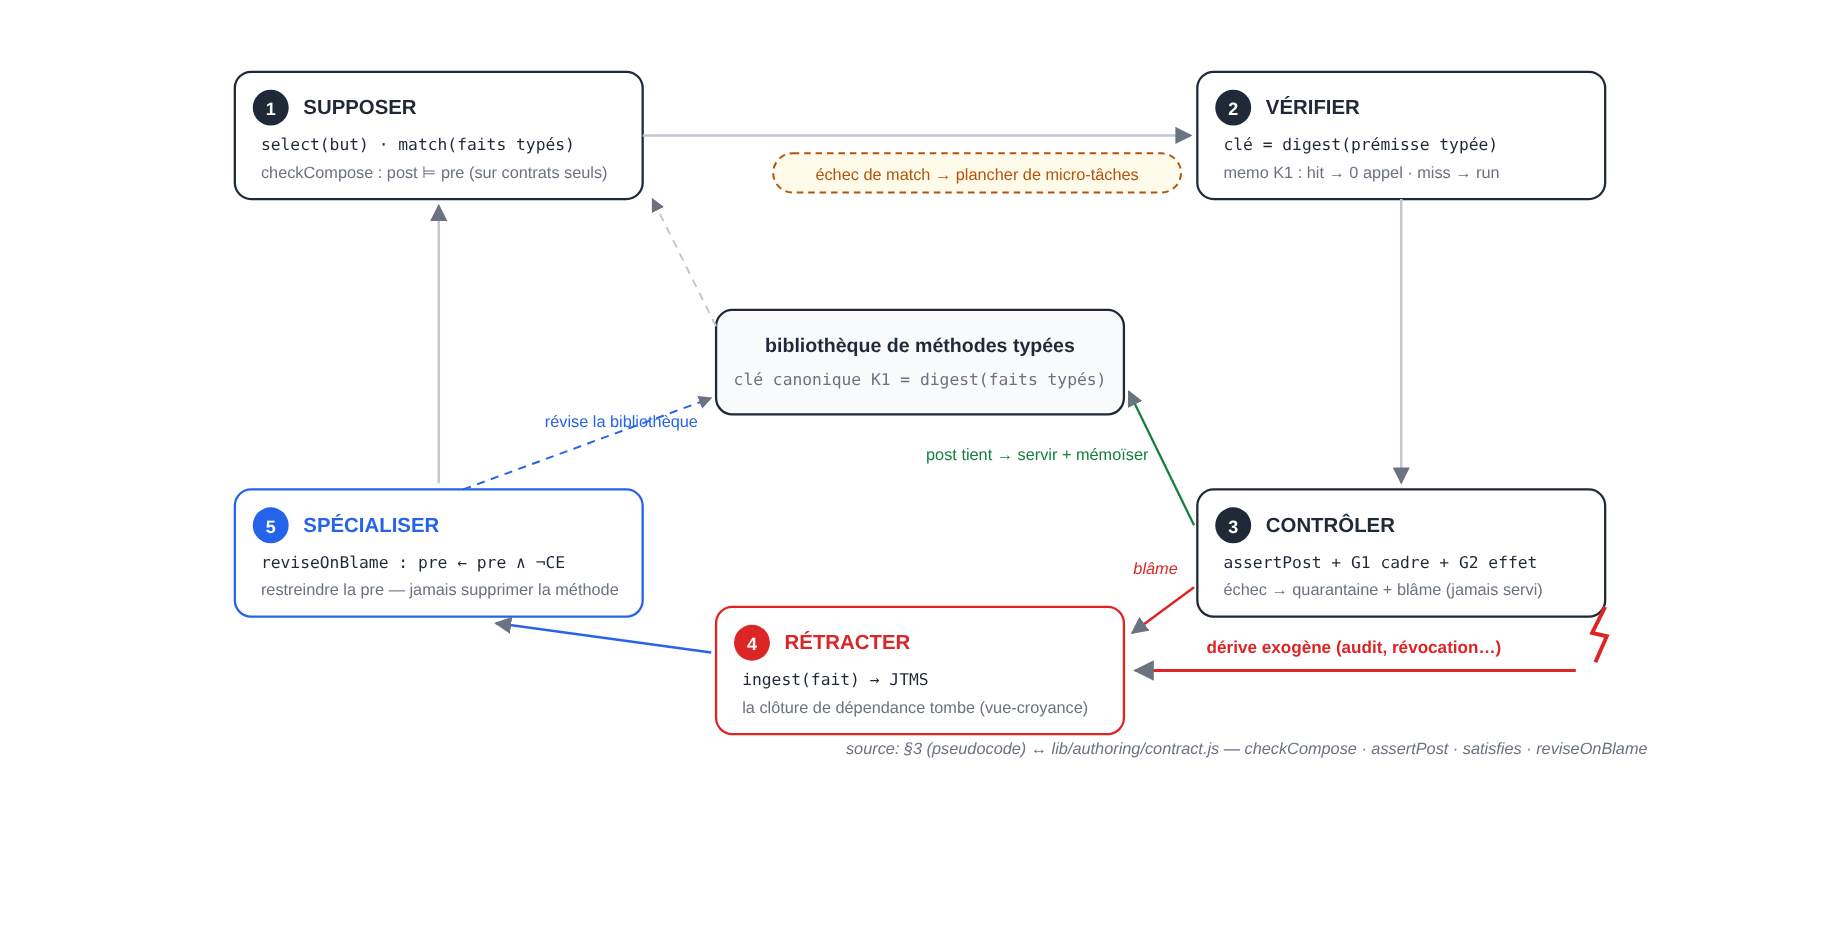
\includegraphics[width=\linewidth]{../figures/png/f2-defeasible-loop.fr.png}
\caption*{\small Figure F2 — le cycle de vie défaisable, en correspondance un-à-un avec les fonctions du moteur : supposer (\texttt{checkCompose}), vérifier (la clé canonique K1 et son mémo), contrôler (\texttt{assertPost} plus les barrières de cadre et d'effet), rétracter (le JTMS, quand la dérive exogène fait tomber une prémisse), spécialiser (\texttt{reviseOnBlame}). L'échec de sélection retombe au plancher de micro-tâches.}
\end{figure}

\medskip\hrule\medskip

\section*{4. Expériences}

Le parcours d'évaluation : le dispositif partagé (§4.1), puis le test décisif de la défaisance à la dérive (E2, §4.2), l'amortissement et le transfert sains (E1, §4.3), la sûreté de composition (E3, §4.4), le plafond de couverture K1 (P4, §4.5), l'échelle (E5, §4.6), le tête-à-tête face aux systèmes nommés (E6, §4.7), la composition à la dérive (E7, §4.8) et la révision de bibliothèque (E8, §4.9). Chaque expérience ouvre sur la promesse de §1 qu'elle contrôle.

\subsection*{4.1 Dispositif}

Les expériences tournent sur le moteur réel ; le modèle fonctionne soit comme \textbf{simulateur déterministe} (un oracle parfait de la règle \emph{courante} étant donné uniquement ce que révèle l'invite de chaque bras — toute péremption et tout coût proviennent donc du mécanisme du bras, non d'une erreur du modèle), soit comme \textbf{modèle local réel} : Qwen3.6-27B, quantisé 2 bits (Q2\_K\_XL), servi avec prédiction multi-token (MTP). Un constructeur d'invite partagé rend le contexte par appel comparable entre bras. Chaque exécution comparative est conditionnée par un \textbf{auto-test du banc} : sous le simulateur le bras naïf doit être parfaitement correct, sinon l'instrumentation est cassée et l'exécution est avortée. Tous les résultats simulés sont déterministes au rejeu. \textbf{Une précision de fidélité s'impose :} E1 et E3 \textbf{instancient le moteur complet} (graphe + stabilisation + JTMS) ; E2, P4 et E5 \textbf{isolent les fonctions} réelles du moteur (\texttt{digest}, \texttt{satisfies}, \texttt{canonValue}) depuis un banc, sans la boucle de stabilisation — nous ne prétendons pas qu'E2 exerce la rétractation JTMS native (il la ré-implémente sur le même prédicat réel). Sept bras partagent une interface :

\begin{itemize}
\item \textbf{Naïf}, \textbf{Long-contexte}, \textbf{RAG} — les références évidentes ;
\item \textbf{CBR} — clé typée, sans re-vérification ;
\item \textbf{Compétence} — des compétences en prose, à la Voyager ;
\item \textbf{Invalidant} — la référence ÉQUITABLE : cache à clé typée plus un rappel grossier codé à la main, qui jette toute une classe auditée à l'événement d'audit — un crochet d'invalidation, mais pas de contrat typé ;
\item \textbf{Struct} — la bibliothèque typée au contrat défaisable : elle re-vérifie la post par entrée, n'évinçant que ce qui est violé.
\end{itemize}

Le bras Invalidant existe pour séparer « possède un mécanisme d'invalidation » de « possède un contrat défaisable typé ».

\subsection*{4.2 E2 — défaisance à la dérive (le test décisif)}

Un domaine d'approbation typé (N = 80, deux classes auditées ; l'exécution réelle utilise N = 48, une classe auditée) avec une invalidation de prémisse \emph{externe} en cours de flux : un audit de conformité marque une classe non conforme, faisant basculer ses cas auparavant approuvés vers le refus. L'audit n'est \textbf{pas un champ d'enregistrement} — il est exogène — donc un cache par rappel seul retrouve le même enregistrement inchangé et sert sa réponse pré-audit. Voici les résultats simulés :

\begin{center}\small\begin{adjustbox}{max width=\linewidth}\begin{tabular}{>{\raggedright\arraybackslash}p{0.299\linewidth}>{\raggedright\arraybackslash}p{0.061\linewidth}>{\raggedright\arraybackslash}p{0.153\linewidth}>{\raggedright\arraybackslash}p{0.184\linewidth}>{\raggedright\arraybackslash}p{0.153\linewidth}}\toprule
bras & appels & exactitude globale & \textbf{exactitude à la dérive} & contexte/appel max \\ \midrule
\textbf{Struct} (contrat typé) & \textbf{26} & \textbf{1.00} & \textbf{1.00} & \textbf{290} \\
Invalidant (crochet, sans contrat) & 28 & 1.00 & 1.00 & 290 \\
Naïf & 80 & 1.00 & 1.00 & 290 \\
Long-contexte & 80 & 1.00 & 1.00 & 2062 \\
RAG & 48 & 0.95 & 0.00 & 290 \\
CBR (clé typée, sans re-vérification) & 24 & 0.95 & 0.00 & 290 \\
Compétence (prose) & 80 & 0.95 & 0.00 & 297 \\
\bottomrule\end{tabular}\end{adjustbox}\end{center}

La lecture est triple. \textbf{Les mémoires par rappel seul (RAG / CBR / Compétence) servent du périmé} — le rappel seul ne récupère pas, l'audit n'entrant jamais dans leur chemin de réutilisation. \textbf{La récupération exige un mécanisme d'invalidation}, et l'Invalidant comme Struct en ont un, donc tous deux atteignent 1.00. Ce que le \textbf{contrat défaisable typé ajoute au rappel codé à la main} tient en trois propriétés :

\begin{itemize}
\item la \textbf{sélectivité} — Struct re-vérifie la post par entrée (\texttt{satisfies}) et n'évince que les 2 classes \emph{violées} (approve), là où le rappel jette grossièrement des classes entières (4 entrées) et paie les re-dérivations supplémentaires (26 vs 28 appels) ;
\item la \textbf{généralité} — le même \texttt{assertPost}, agnostique-à-la-prémisse par construction (les expériences n'exercent qu'un seul type de prémisse, un basculement de drapeau de conformité), tandis que le rappel est codé à la main par événement ;
\item la \textbf{sûreté de composition} (§4.4). L'exécution réelle (Qwen3.6-27B (Q2\_K\_XL,
\end{itemize}
MTP), N = 48) reproduit ce classement : RAG/CBR/Compétence 0.00 ; Invalidant 14 appels / 1.00 ; Struct 13 appels / 2,6 s / 1.00 / ctx 278 vs Long-contexte 1304.

\begin{figure}[htbp]\centering
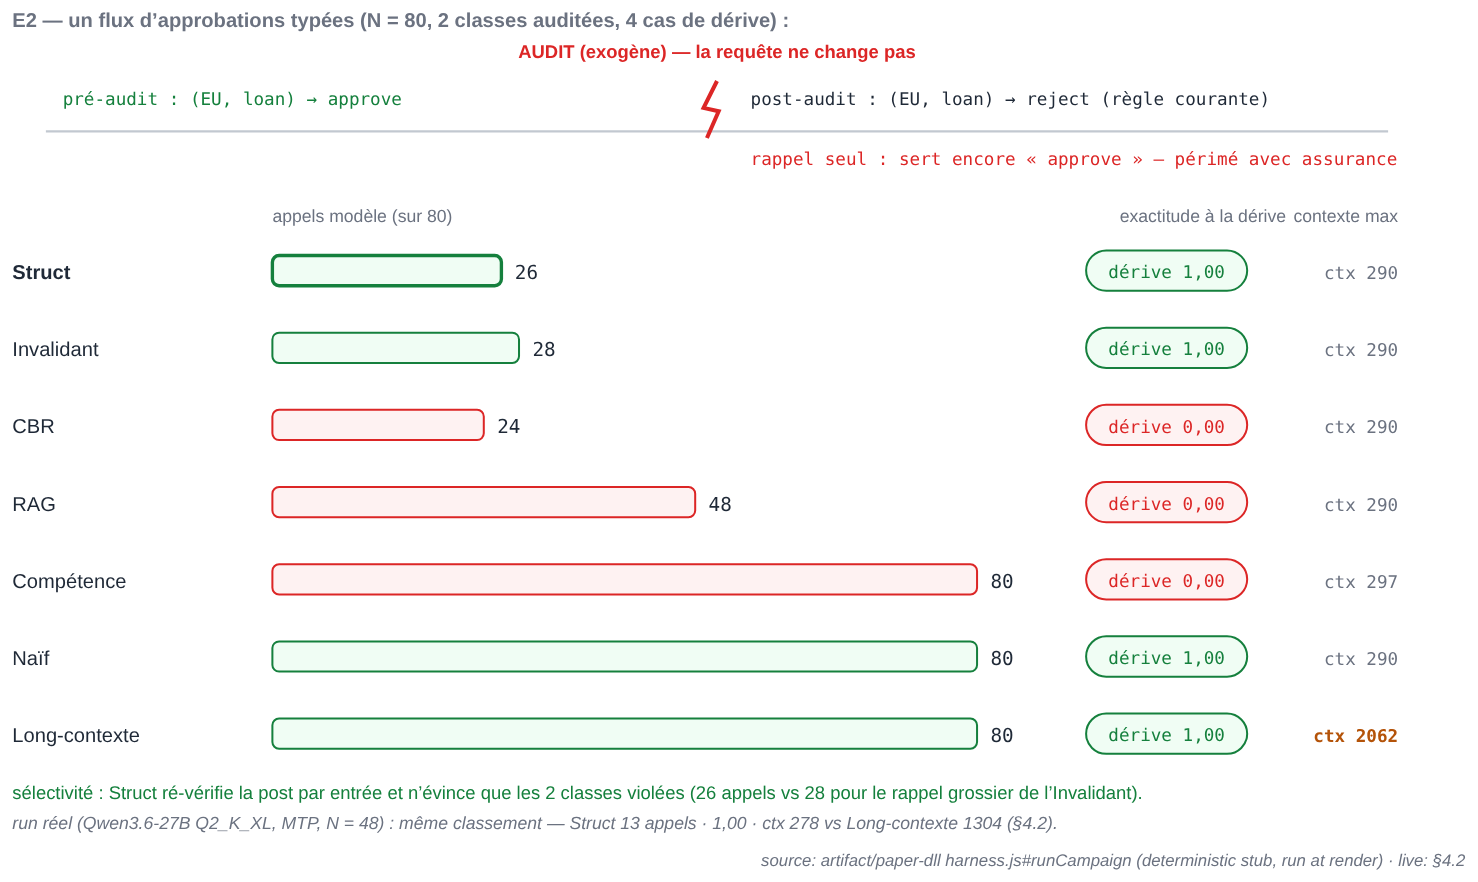
\includegraphics[width=\linewidth]{../figures/png/f3-e2-drift.fr.png}
\caption*{\small Figure F3 — E2 : l'audit exogène bascule une classe en cours de flux sans changer la requête. Les mémoires par rappel seul (rouge) servent du périmé ; les bras à invalidation (vert) récupèrent ; le contrat typé récupère sélectivement (26 appels, 2 évictions — les seules classes violées). Barres, verdicts et comptes recalculés au rendu depuis le harnais déterministe de l'artefact.}
\end{figure}

L'affirmation défendable n'est donc pas « seul Struct récupère » mais « la mémoire par rappel seul ne sait pas désapprendre, et un contrat typé déclaratif fournit la récupération de façon sélective, générale et sûre en composition ».

\subsection*{4.3 E1 — amortissement et transfert structurel}

E2 a montré la récupération à la dérive ; l'autre promesse de §1 — une réutilisation qui amortit \emph{sans rejouer faux} — se contrôle ici. Le banc : un domaine de décomposition structurelle (une méthode qui \emph{crée} un sous-graphe avec des identifiants d'objets), sur le \textbf{moteur complet}. La partition : entraînement, \textbf{apparentés tenus à l'écart} (mêmes transitions typées, espaces d'identifiants frais) et \textbf{nouveau tenu à l'écart}. C'est un contrôle d'\textbf{existence-et-sûreté sur un petit ensemble} (2 apparentés, 1 nouveau), \textbf{pas un taux de population} : avec la transformation relativiser/lier, \emph{toutes} les instances apparentées tenues à l'écart transfèrent à 0 appel et \textbf{sainement}, tandis que la transition nouvelle paie son appel (pas de faux rejeu) — au total 3 appels contre 5 pour la référence sans cache. L'ablation sans transformation (un cache de contenu plat) « touche » les problèmes apparentés mais rejoue le \emph{mauvais espace d'identifiants} — \textbf{non sain}.

Le point est qualitatif : une métrique fondée sur le seul nombre d'appels classe le cache plat à égalité avec la transformation (les deux éludent) ; \textbf{seule la vérification de sûreté} distingue une réutilisation saine d'un rejeu dans le mauvais espace d'identifiants. (Étendre cela à un \emph{taux} de transfert sur de nombreuses méthodes est un travail futur.)

\subsection*{4.4 E3 — sûreté de composition}

Troisième promesse de §1 : composer sans ouvrir la boîte. En composant des paires de méthodes sur leurs seuls contrats typés (boîte fermée) et en comparant au résultat moteur boîte ouverte (sur le \textbf{moteur complet}), la décision boîte fermée \textbf{coïncide avec la réalité sur chaque paire évaluée, sans faux-admis} — le vérificateur n'accepte jamais à tort ; les paires sous-déterminées ou hors-fragment \emph{escaladent} (vers une micro-tâche) plutôt que d'admettre. C'est démontré sur un petit ensemble construit à la main (3 paires couvrant sain / non-sain / escalade ; une 4ᵉ ajoute le cas oracle) : une \textbf{démonstration d'existence} de la sûreté, \textbf{pas un taux} de faux-admis de population.

Chacune des trois barrières est porteuse sur un exemple dédié : retirer la complétude de cadre manque une écriture non déclarée ; retirer l'étiquette d'effet admet silencieusement un effet externe non vérifié ; retirer la détection de cycle d'empreintes admet un cycle couplé rétractable. La décision ne lit que l'empreinte partagée, jamais le corps ; le vérificateur lui-même (implication par domaines abstraits, sain-mais-incomplet) est l'artefact le plus développé et plutôt sous-évalué ici. (Un corpus plus grand, non trié à la main, est un travail futur.)

\subsection*{4.5 P4 — le plafond de couverture K1}

Reste la contrainte K1 annoncée en §1 : que coûte-t-elle réellement ? Sur une charge mixte (fraction \emph{p} entièrement typée ; le reste portant un composant en prose qui prime sur la règle typée), l'appartenance à K1 étant décidée par la \textbf{vraie} barrière de canonicalisation, l'amortissement est un \textbf{gradient en couverture} (approbation : 0 → 19 → 44 → 69 → 94 \% élidé à p = 0/0,25/0,5/0,75/1 ; tri : 0 → 22 → 47 → 72 → 97 \%). L'exactitude de Struct est \textbf{1.00 à chaque couverture} — la fraction non typée est un \emph{coût} de micro-tâche, jamais une \emph{falaise} de sûreté. Une variante gloutonne qui mémoïse les enregistrements porteurs de prose sur leur clé typée chute à une exactitude égale à la fraction propre : \textbf{amortir au-delà de la fraction canonicalisable est non sain}, donc le plafond K1 est une \emph{frontière de sûreté}, pas une optimisation manquée. Le résultat tient sur les deux domaines et est déterministe. Nous sommes explicites : c'est une \textbf{illustration construite}, pas une mesure sur charge réelle — nous \emph{fixons} p et \emph{définissons} les enregistrements en prose pour primer sur la règle typée, donc « amortir au-delà de K1 est non sain » découle par construction. Ce qu'elle établit, c'est la \emph{forme} (amortissement proportionnel à la couverture) et la sûreté à chaque niveau ; la fraction canonicalisable d'un corpus réel est dépendante du domaine et non mesurée ici.

\begin{figure}[htbp]\centering
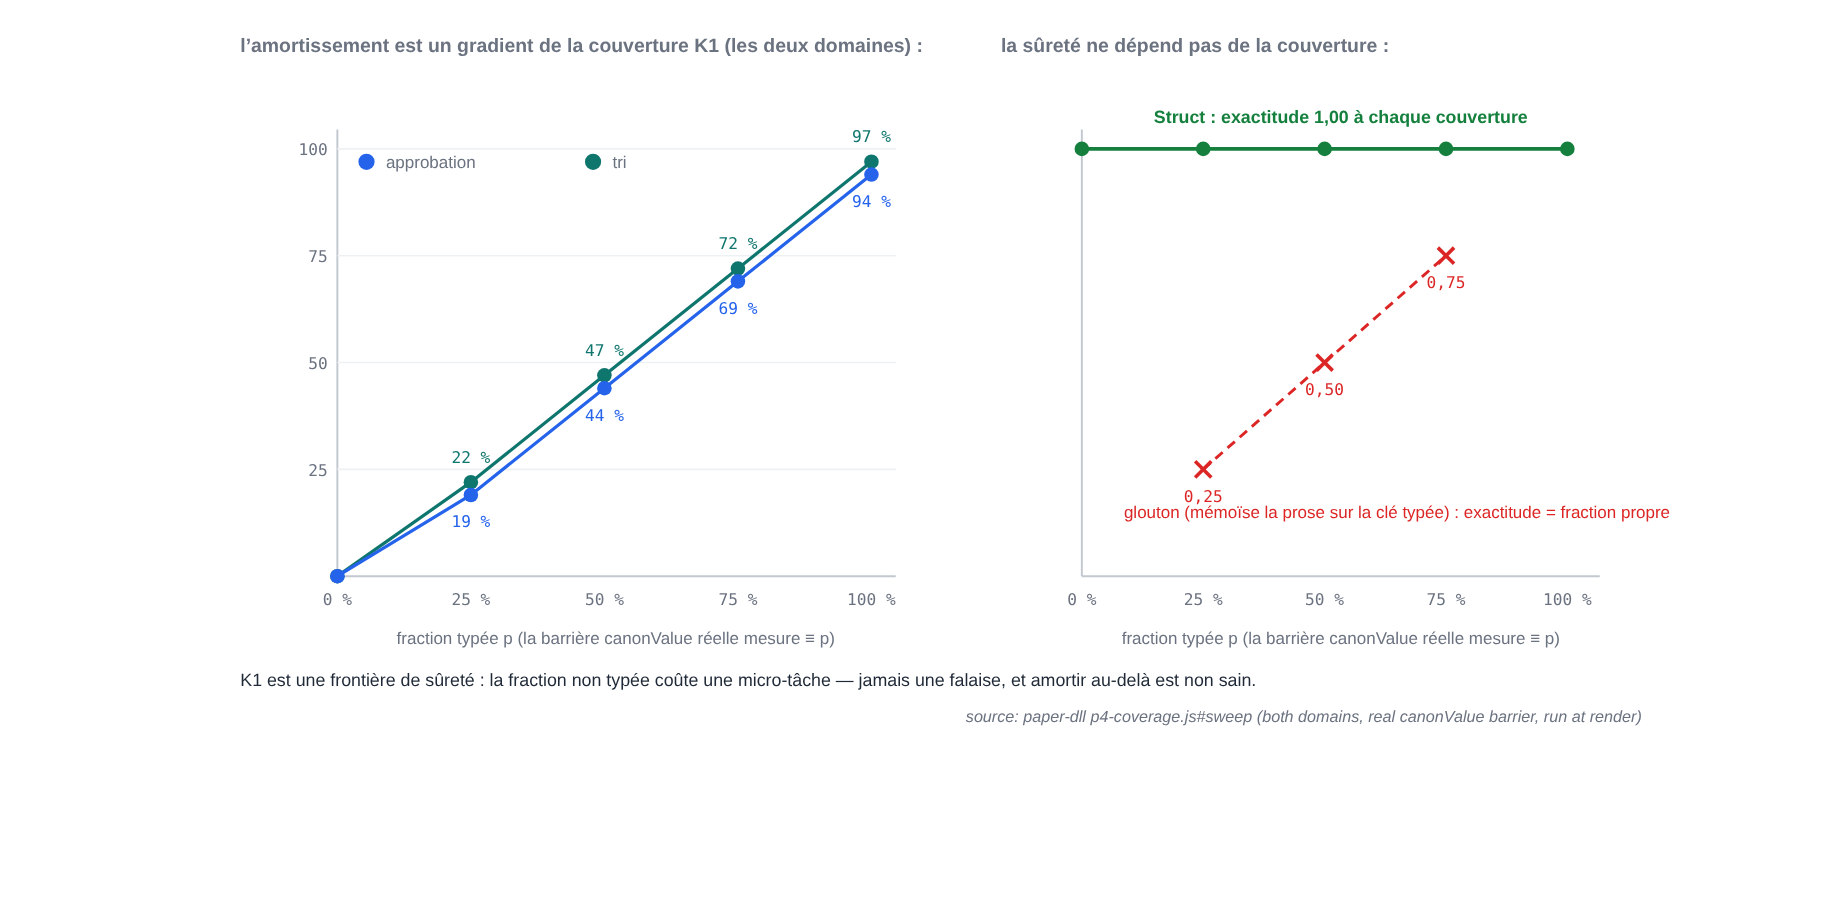
\includegraphics[width=\linewidth]{../figures/png/f6-p4-k1.fr.png}
\caption*{\small Figure F6 — P4 : l'amortissement est un gradient de la couverture K1 (à gauche, les deux domaines) ; la sûreté n'en dépend pas (à droite : 1,00 à chaque couverture, tandis que le contrôle négatif glouton chute à la fraction propre). K1 est une frontière de sûreté, pas une optimisation manquée.}
\end{figure}

\subsection*{4.6 E5 — passage à l'échelle et coût par mécanisme}

Un contrôle de \textbf{coût de tenue de registre}, pas une affirmation sur le passage à l'échelle de la partie difficile — une bibliothèque de méthodes \emph{distinctes} qui croît, laissée en travaux futurs (fin de section) : sur un espace typé de 200 classes avec un audit unique, quand la longueur du flux N croît de 1 320 à 20 320 (l'\emph{ensemble des classes} est fixe ; aucune nouvelle méthode, aucun modèle) :

\begin{center}\small\begin{adjustbox}{max width=\linewidth}\begin{tabular}{llllll}\toprule
N & appels Struct & appels / N & appels Naïf & bibliothèque (mémo) & évincés à la dérive \\ \midrule
1 320 & 202 & 0,153 & 1 320 & 200 & 2 \\
5 320 & 202 & 0,038 & 5 320 & 200 & 2 \\
20 320 & 202 & 0,010 & 20 320 & 200 & 2 \\
\bottomrule\end{tabular}\end{adjustbox}\end{center}

Le nombre d'appels de Struct reste \textbf{constant} (le nombre borné de classes distinctes plus les re-dérivations de dérive), donc le taux d'appels par enregistrement tend vers zéro tandis que Naïf reste à un ; la \textbf{bibliothèque est bornée} par le nombre de classes, indépendamment de N ; et un événement de dérive \textbf{ne rétracte que les classes invalidées} (2 évictions sur une bibliothèque de 200 entrées — O(invalidé), pas O(bibliothèque)). Les coûts par opération sont faibles : la canonicalisation est de quelques µs par appel (dépend de l'environnement), et une passe d'éviction de dérive ≈ 0,5 ms sur toute la bibliothèque. Le contenu honnête est étroit : la tenue de registre typée ne devient pas le goulet d'étranglement quand le flux croît. Cette expérience ne teste en revanche \textbf{pas} le passage à l'échelle dans la dimension qui compte — une bibliothèque croissante de méthodes \emph{distinctes}, un corpus réel, ou un modèle réel sur tous les bras — qui reste en travaux futurs.

\subsection*{4.7 E6 — tête-à-tête face aux systèmes de mémoire d'agents nommés}

Les références de §4.1 sont génériques (RAG / CBR / Compétence). Les systèmes qu'un relecteur attend en comparaison sont les systèmes \emph{nommés} : \textbf{MemGPT/Letta} (contexte virtuel à étages, mémoire auto-éditée) [Packer et al. 2023], \textbf{Reflexion} (un essai-réflexion verbale épisodique piloté par un signal d'échec) [Shinn et al. 2023], et \textbf{GraphRAG} (un index de graphe de connaissances hors-ligne avec résumés de communautés par LLM) [Edge et al. 2024]. Nous ajoutons une ré-implémentation minimale fidèle de chacun de ces trois systèmes, derrière la même interface et dans sa configuration \emph{la plus favorable}, avec une ablation appariée qui éteint son mécanisme distinctif (le contrôle négatif). Le banc est un stub déterministe : N = 78, deux classes auditées, six cas de dérive :

\begin{center}\small\begin{adjustbox}{max width=\linewidth}\begin{tabular}{lllll}\toprule
bras & appels modèle & exact. & exact.-dérive & ctx max \\ \midrule
Naïf & 78 & 1,00 & 1,00 & 290 \\
\textbf{MemGPT} (audit paginé en core) & 23 & 1,00 & 1,00 & 320 \\
MemGPT − pagination (ablation) & 18 & 0,92 & 0,00 & 258 \\
\textbf{Reflexion} (signal d'échec différé) & 82 & 1,00 & 1,00 & 332 \\
Reflexion − signal (ablation) & 78 & 0,92 & 0,00 & 258 \\
\textbf{GraphRAG} (index hors-ligne) & 87 & 0,92 & 0,00 & 336 \\
GraphRAG + ré-index (ablation) & 89 & 1,00 & 1,00 & 336 \\
\textbf{Struct} & \textbf{20} & \textbf{1,00} & \textbf{1,00} & \textbf{290} \\
\bottomrule\end{tabular}\end{adjustbox}\end{center}

\begin{figure}[htbp]\centering
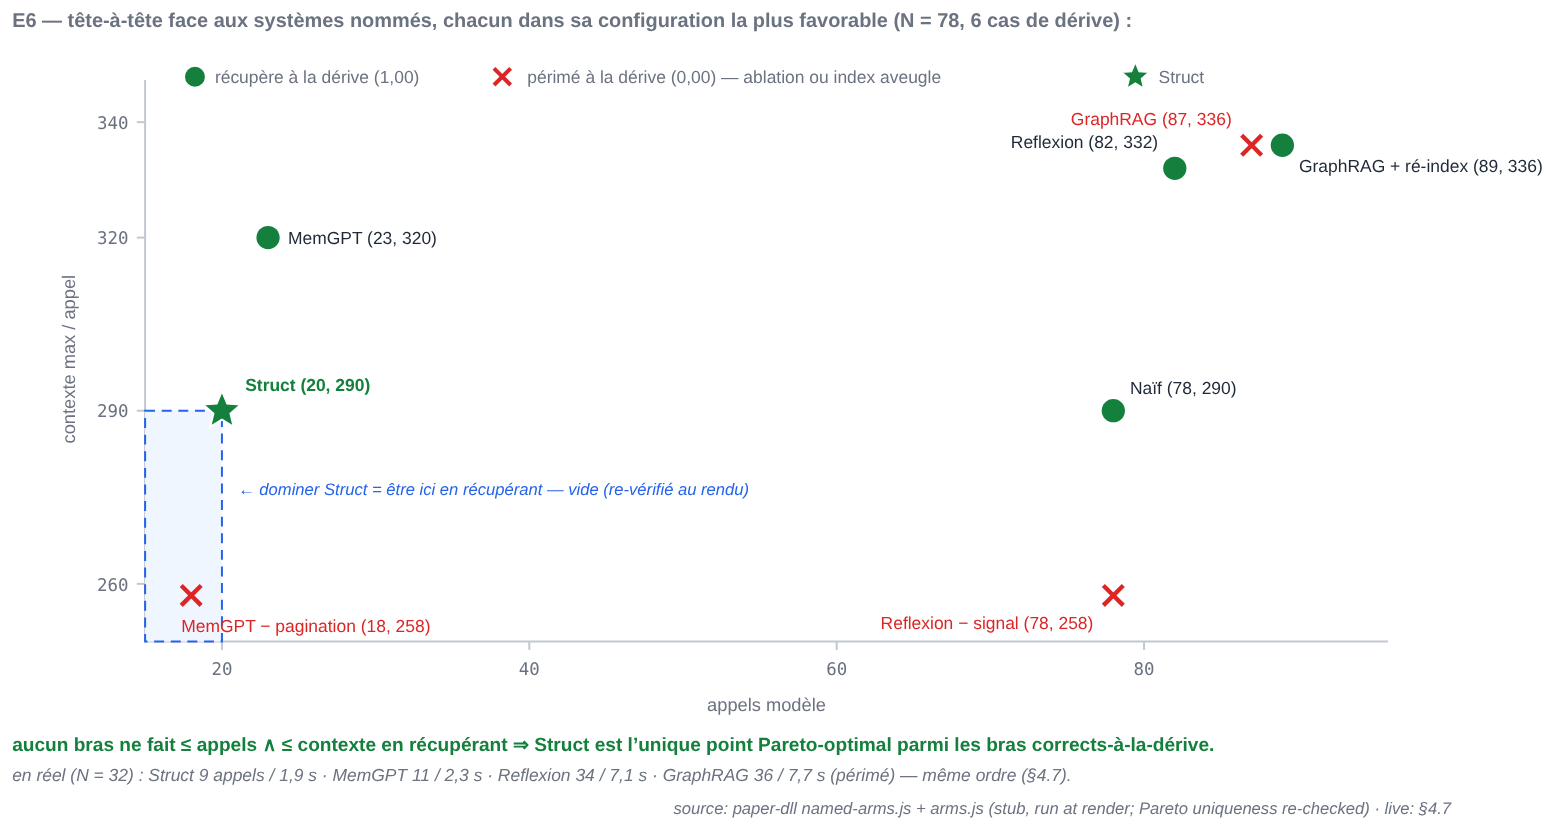
\includegraphics[width=\linewidth]{../figures/png/f4-e6-pareto.fr.png}
\caption*{\small Figure F4 — E6 sur le plan (appels × contexte par appel) : vert = récupère à la dérive, rouge = périmé. La zone en pointillés — faire ≤ appels et ≤ contexte que Struct — est vide parmi les bras qui récupèrent : Struct est l'unique point Pareto-optimal, unicité re-vérifiée au rendu.}
\end{figure}

La lecture honnête n'est \emph{pas} « seul Struct récupère » : dans sa configuration la plus favorable, chaque système nommé \textbf{peut} récupérer l'exactitude à la dérive (MemGPT et Reflexion atteignent exact.-dérive 1,00 ; GraphRAG dès qu'il ré-indexe).

Le propos est que Struct récupère au moindre coût sur les trois axes \emph{à la fois} — c'est le seul bras qui récupère à la dérive tout en restant non-dominé (aucun bras ne l'égale-ou-bat sur les appels ET le contexte par appel tout en récupérant ; les bras moins chers sont sur la frontière de coût mais échouent à la dérive). Chaque système nommé paie une taxe propre à son mécanisme :

\begin{itemize}
\item \textbf{MemGPT} ne récupère qu'une fois l'audit exogène fait surface et auto-édité en mémoire core (un tour modèle) ; la récupération est alors \emph{grossière} — un drapeau de classe (region,kind) entière qui re-décide même les membres à faible score non concernés (sur-éviction, +appels) — et un bloc de mémoire core voyage dans chaque invite (+contexte).
\item \textbf{Reflexion} n'a \emph{aucun mémo adressé par contenu}, donc il émet un appel modèle sur \textbf{chaque} enregistrement (appels ≈ N — l'écart décisif), et ne récupère que \emph{réactivement}, après un échec observé, via une réflexion en prose stockée (un retard de récupération + du contexte préfixé).
\item L'index hors-ligne de \textbf{GraphRAG} est aveugle à l'audit silencieux, donc périmé par défaut ; la récupération exige un \textbf{ré-résumé par lot} des communautés concernées (grossier, par communauté, hors-bande), jamais un défaiseur par entrée. (GraphRAG est hors de son domaine de conception pour des décisions ponctuelles — sa force est la synthèse globale ; ceci éprouve le système de recherche-par-graphe nommé sur l'axe de la défaisance.)
\end{itemize}

Les systèmes nommés n'ont pas été conçus pour amortir des décisions ponctuelles typées récurrentes ; cette charge les éprouve hors de leur domaine de conception, de sorte que la « taxe » est le coût d'un outil inadapté, non une infériorité à leur propre tâche. Les ablations confirment que chaque mécanisme est porteur (éteint → exact.-dérive 0,00). Mesurée \emph{en isolation} (appels sur le flux dérivant moins appels sur un jumeau sans dérive), la taxe de récupération de Struct est la re-dérivation des seules entrées \textbf{violées} (2 ; sélectif), et la ré-assertion du contrat est elle-même intra-moteur — \textbf{zéro} appel modèle — strictement sous celle de chaque système nommé. Un essai en direct (Qwen3.6-27B (Q2\_K\_XL, MTP), N = 32) reproduit l'ordre : Struct \textbf{9} appels / 1,9 s, MemGPT 11 / 2,3 s, Reflexion 34 / 7,1 s, GraphRAG 36 / 7,7 s (périmé) ; Struct est l'unique point Pareto-optimal parmi les bras corrects-à-la-dérive en direct aussi. Ce sont des ré-implémentations minimales fidèles de chaque mécanisme, pas les systèmes complets (§6).

\subsection*{4.8 E7 — composition à la dérive}

E6 mesure une \emph{seule} méthode. Le différenciateur d'une \emph{bibliothèque} est la composition : lorsque la prémisse d'une méthode amont tombe, la récupération se propage-t-elle dans la chaîne ? Nous étendons la charge à une chaîne à deux maillons — \texttt{decide → disburse}, où \texttt{disbursement = disbursed iff decision == approve} (le maillon 2 lit le fait-résultat du maillon 1) — et ré-exécutons le tête-à-tête en notant les \textbf{deux} maillons. Le même audit exogène se propage désormais en cascade : un cas audité à score élevé doit faire basculer \texttt{decision} approve→reject \textbf{et} \texttt{disbursement} disbursed→held. Deux régimes sont courus : le simulateur déterministe (N = 78, deux classes auditées) et une exécution réelle (Qwen3.6-27B (Q2\_K\_XL, MTP), N = 48) :

\begin{center}\small\begin{adjustbox}{max width=\linewidth}\begin{tabular}{>{\raggedright\arraybackslash}p{0.264\linewidth}>{\raggedright\arraybackslash}p{0.187\linewidth}>{\raggedright\arraybackslash}p{0.213\linewidth}>{\raggedright\arraybackslash}p{0.213\linewidth}}\toprule
bras & appels (simu / réel) & exact.-dérive maillon 1 & exact.-dérive maillon 2 \\ \midrule
Naïf & 156 / 96 & 1,00 & 1,00 \\
CBR (= Struct − contrat) & 36 / 24 & \textbf{0,00} & \textbf{0,00} \\
MemGPT (le plus favorable) & 45 / 41 & 1,00 & 1,00 \\
Reflexion (le plus favorable) & 160 / 108 & 1,00 & 1,00 \\
GraphRAG + ré-index & 178 / 116 & 1,00 & 1,00 \\
\textbf{Struct} & \textbf{38 / 26} & \textbf{1,00} & \textbf{1,00} \\
Struct (moteur complet) & 38 / 27 & 1,00 & 1,00 \\
\bottomrule\end{tabular}\end{adjustbox}\end{center}

Trois choses sont mesurées. (i) \textbf{La péremption se cumule.} Tout bras par rappel seul ou aveugle (CBR, et l'ablation de chaque système nommé) est faux au maillon 1 \emph{et} au maillon 2 : une réponse amont périmée empoisonne le maillon aval qui la lit. L'exactitude à la dérive est mesurée sur l'oracle déterministe ; l'exécution réelle confirme l'ordre des appels et du temps (le modèle réel est imparfait à petit N, nous ne lisons donc pas la dérive par enregistrement sur lui). (ii) \textbf{La taxe de récupération se multiplie le long de la chaîne.} Reflexion, sans mémo, paie un appel par enregistrement \emph{par maillon} (appels ≈ 2N) ; GraphRAG ré-indexe les communautés concernées à \emph{chaque} maillon ; MemGPT paie la pagination + un re-décodage grossier + un contexte plus grand aux \emph{deux} maillons. (iii) \textbf{La cascade de Struct est sélective.} Une prémisse tombée dé-cast la croyance amont et le changement se propage à l'aval — récupérant les deux maillons tout en re-dérivant \emph{seulement} l'entrée amont violée (la re-dérivation aval est élidée car sa clé de cache est l'ensemble de lecture réel de disburse \texttt{\{kind, region, decision\}}). Struct est l'unique point Pareto-optimal parmi les bras corrects-à-la-dérive sur (appels × exact.-dérive maillon 1 × exact.-dérive maillon 2 × contexte par appel), en simu comme en réel ; la réalisation sur moteur complet (quatre concepts \emph{ensure}-gated au-dessus du cache de dérivation) la reproduit (38 = 38 en simu ; 26 ≈ 27 en réel, dans le non-déterminisme du modèle).

\begin{figure}[htbp]\centering
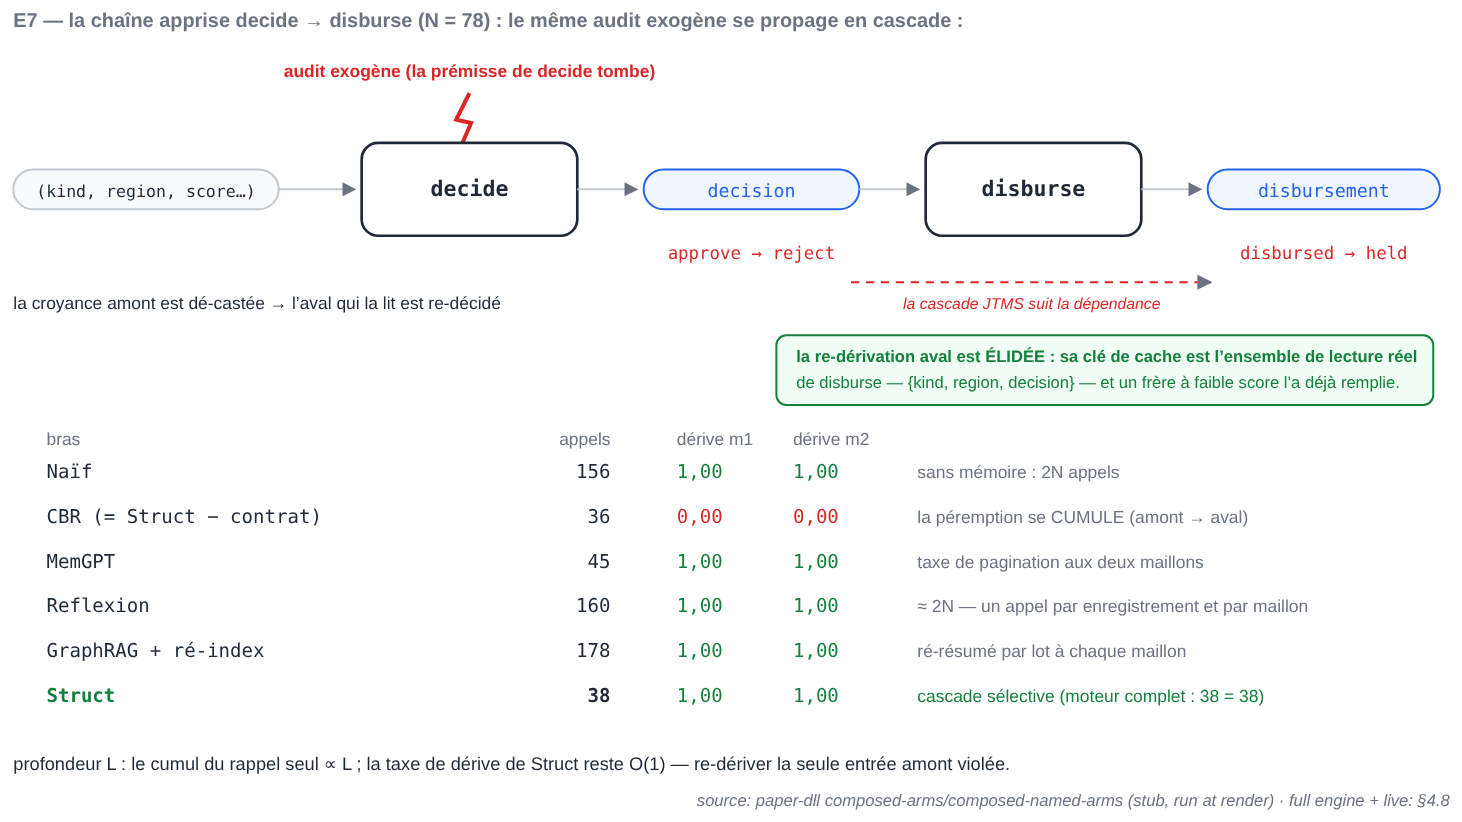
\includegraphics[width=\linewidth]{../figures/png/f5-e7-cascade.fr.png}
\caption*{\small Figure F5 — E7 : la dérive à travers la chaîne apprise decide → disburse. La prémisse amont tombe ; la cascade JTMS rétracte la décision et le versement qui la lit ; seule l'entrée amont violée est re-dérivée — la re-dérivation aval est élidée par sa clé d'ensemble-de-lecture, déjà remplie par un frère. Table recalculée au rendu.}
\end{figure}

C'est la capacité qui manque structurellement aux mémoires de surface nommées : une croyance qui dépend d'une prémisse qui vient de tomber, désapprise \emph{à travers la composition}.

\textbf{L'avantage s'élargit avec la profondeur de chaîne.} Généralisons la chaîne à L maillons, chacun positif ssi le précédent l'est. La péremption et le coût croissent alors tous deux avec L, mais pas la récupération de Struct : la \emph{profondeur de cumul} d'un cache par rappel seul (le nombre de maillons faux sur une classe dérivée) vaut exactement L ; Naïf et Reflexion paient O(L·N) appels ; la \emph{taxe de dérive} de Struct, elle, est en \textbf{O(1) en L} — la cascade ne re-dérive que l'entrée amont violée, chaque re-dérivation aval réutilisant l'entrée d'ensemble-de-lecture d'un frère. Plus la chaîne de méthodes apprises est profonde, plus l'avantage de Struct est donc grand : sur l'exactitude (le cumul ∝ L) et sur l'efficacité de récupération (O(1) contre une reconstruction grossière en O(L)). Deux conditions de validité, dites : la récupération en O(1) tient lorsque chaque re-dérivation aval retombe sur une clé de cache qu'un frère a déjà remplie — vrai ici, la branche négative étant partagée et pré-remplie par les frères à faible score ; sous un fort éventail aval, la taxe croît vers O(L). Et le cumul ∝ L découle par construction de la définition du maillon \emph{i} comme fonction du maillon \emph{i}−1 ; il est mesuré sur le simulateur déterministe (le balayage en L en réel est confondu par le bruit, §6).

\textbf{Sur le vrai exécuteur durable.} Ce qui précède est la vue-croyance (le graphe à base de règles + la rétractation JTMS). La même chaîne compilée en un réseau de workflow et exécutée comme un flot de jetons sur un magasin de points de reprise adressé par contenu et reprenable après crash reproduit le résultat sur la couche d'\emph{exécution} : la chaîne amortit et la dérive se propage en cascade à travers les deux maillons (Struct-sur-exécuteur 24 appels, dérive 1,00/1,00 ; la clé sans-prémisse comme le cache composé plat y cumulent la péremption), la bibliothèque composée chaude \textbf{se rejoue à travers un redémarrage de processus à zéro appel modèle}, et une chaîne coupée en plein vol \textbf{reprend sans travail perdu ni dupliqué}. La défaisance en vue-croyance et l'exécution durable sont complémentaires : le contrat rétracte la croyance ; l'exécuteur rend le recalcul durable et sélectif.

\subsection*{4.9 E8 — révision de bibliothèque sous dérive récurrente}

E2/E6/E7 mesurent le chemin \emph{rétracter → re-dériver} : une post violée évince la croyance en cache, qui est ensuite re-dérivée. L'autre moitié de la boucle — \emph{réviser} : spécialiser la précondition de la méthode sur blâme, de sorte que la bibliothèque soit améliorée, non simplement ré-évaluée — est évaluée ici. Nous exécutons K = 5 épisodes de dérive récurrente (les mêmes classes reviennent à chaque épisode après qu'une précondition trop générale a été exposée) et comparons l'éviction-seule à la révision via le \texttt{reviseOnBlame} du moteur :

\begin{center}\small\begin{adjustbox}{max width=\linewidth}\begin{tabular}{lll}\toprule
sur K=5 épisodes & Éviction-seule & Révision (\texttt{reviseOnBlame}) \\ \midrule
blâmes (par épisode → cumulatif) & 1,1,1,1,1 → 5 & 1,0,0,0,0 → 1 \\
re-dérivations (appels modèle) & 4,1,1,1,1 → 8 & 4,1,0,0,0 → 5 \\
taux de faux-admis & 0,25 à chaque épisode & 0,25 → 0,00 après e1 \\
\bottomrule\end{tabular}\end{adjustbox}\end{center}

L'éviction-seule conserve la règle trop générale, donc elle ré-admet, re-blâme et re-dérive la même classe périmée à \emph{chaque} épisode (coût ∝ K). La révision spécialise la précondition une seule fois — en la restreignant avec l'atome discriminant du contre-exemple — puis se stabilise : plus aucun blâme, faux-admis → 0. La révision est \emph{chirurgicale} : la précondition spécialisée exclut la classe fautive tout en admettant encore son frère (elle restreint, elle ne supprime pas la méthode). L'effet tient pour deux types de prémisse — un basculement de conformité catégoriel (\texttt{\$compliant != false}) et une porte numérique (\texttt{\$score != 680}). \textbf{Limite honnête :} \texttt{reviseOnBlame} spécialise par exclusion ponctuelle de contre-exemple, non par resserrement de borne ; une dérive numérique couvrant D valeurs distinctes converge en D blâmes ponctuels (bornés, par valeur) plutôt qu'en un seul déplacement de borne — toujours catégoriquement mieux que la récurrence par épisode de l'éviction-seule.

\begin{figure}[htbp]\centering
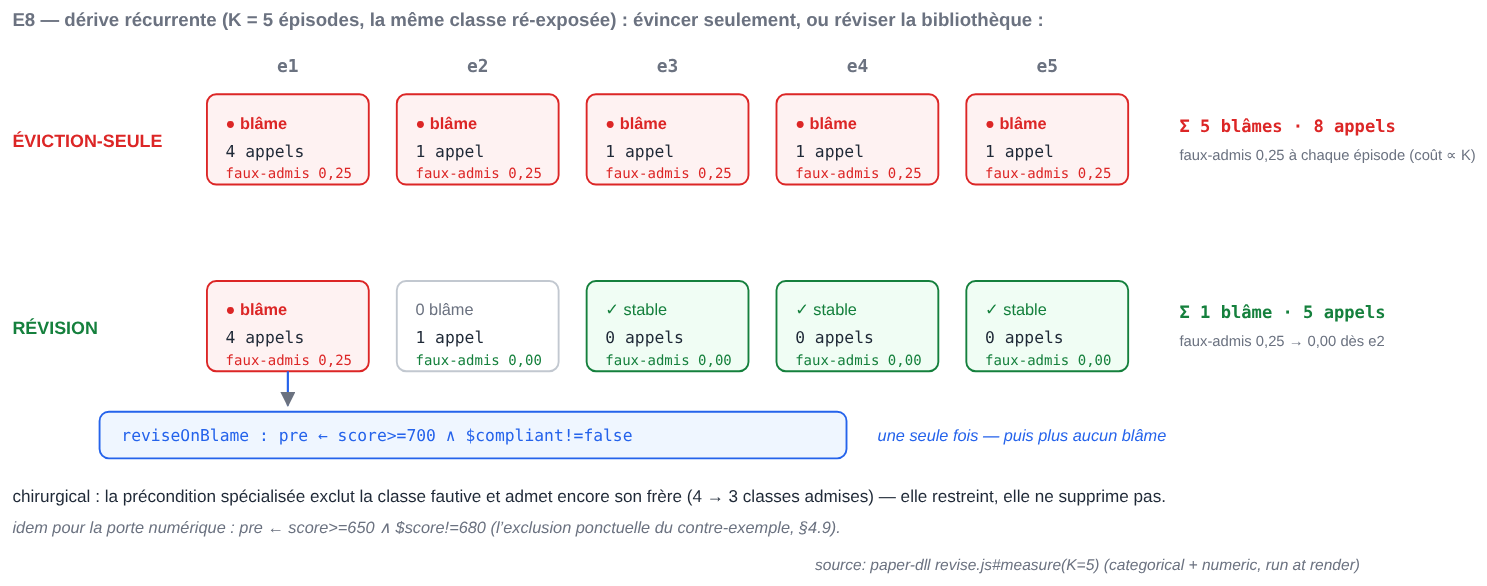
\includegraphics[width=\linewidth]{../figures/png/f7-e8-revision.fr.png}
\caption*{\small Figure F7 — E8 : sous dérive récurrente (K = 5), l'éviction-seule re-blâme et re-paye la même classe à chaque épisode ; la révision spécialise la précondition une seule fois (\texttt{reviseOnBlame}, avec l'atome discriminant réel) puis se stabilise — chirurgicale : le frère reste admis.}
\end{figure}

C'est l'étape qui distingue le contrat de l'invalidation de cache (§5) : le blâme alimente la \emph{révision de bibliothèque}, non le seul recalcul de valeurs.

\medskip\hrule\medskip

\section*{5. Travaux apparentés}

Les voisinages se visitent du plus évident au plus proche : les mémoires par rappel (recherche/cas, puis les mémoires d'agents nommées, puis le long contexte), les bibliothèques apprises, les contrats, les cadres de composition, la révision de théorie — le voisin le plus proche —, le maintien de la vérité, et enfin la plomberie (exécution durable, maintenance de vues) dont nous ne revendiquons rien.

\textbf{Recherche et mémoire de cas.} RAG [Lewis et al. 2020] et CBR [Aamodt \& Plaza 1994] rappellent par similarité de surface/plongement et réutilisent-ou-adaptent ; ils ne peuvent représenter une \emph{prémisse devenant invalide}, donc un changement exogène qui laisse la requête inchangée laisse la réponse en cache retrouvable et périmée (E2). Les bibliothèques de compétences comme Voyager [Wang et al. 2023] stockent des compétences en \emph{prose} sans prémisse typée défaisable, donc une compétence périmée reste applicable et doit être ré-appliquée par le modèle — coût sans exactitude (notre bras Compétence). Notre prémisse typée vit dans la croyance, donc quand elle tombe la dérivation se rétracte (JTMS) et la bibliothèque restreint la méthode.

\textbf{Mémoire des agents LLM.} Les systèmes de mémoire d'agents récents gèrent \emph{ce qu'il faut garder et rappeler} bien plus finement que le RAG ordinaire — le contexte virtuel à étages de MemGPT/Letta [Packer et al. 2023], le tampon épisodique de réflexion verbale de Reflexion [Shinn et al. 2023], et la recherche structurée par graphe comme GraphRAG [Edge et al. 2024]. Mais ils rappellent et réutilisent par pertinence, récence ou similarité et, à notre connaissance, aucun ne représente une \emph{prémisse typée dont la falsification rétracte une réutilisation antérieure}. Ces systèmes sont complémentaires plutôt que concurrents : un contrat défaisable pourrait se placer sous chacun d'eux comme couche de rétractation. Nous menons ce tête-à-tête en \textbf{§4.7 (E6)} : chacun, dans sa configuration la plus favorable, peut récupérer à la dérive, mais seul le contrat défaisable le fait au moindre coût sur (appels × exactitude × contexte) simultanément — les autres paient une taxe de pagination / par-enregistrement / de ré-index par lot.

\textbf{Long contexte.} Porter tout l'historique par appel est correct mais en O(N) de contexte par appel (E2 : 2062 contre 290) sans réutilisation structurelle.

\textbf{Apprentissage de bibliothèque / EBL.} DreamCoder [Ellis et al. 2021] et Stitch [Bowers et al. 2023] font croître une bibliothèque par abstraction (anti-unification / MDL [Plotkin 1970]) ; l'EBG [Mitchell, Keller \& Kedar-Cabelli 1986] spécialise à partir d'une seule preuve. Ils apprennent \emph{quoi} réutiliser mais n'attachent aucun contrat d'exécution défaisable qui se désapprend à la dérive ; nous ajoutons ce contrat et sa révision pilotée par le blâme.

\textbf{L'article compagnon : l'admission des unités apprises.} Le présent article suppose que ce qui entre dans la bibliothèque a été admis sainement depuis des épisodes LLM bruités. Ce problème d'admission — rendre l'élimination de candidats tolérante au bruit d'incompétence d'un LLM par une porte à attribution localisée, appliquée aux grains restriction de slot, arête \emph{isa} et alias de surface — est traité et mesuré dans [Braun 2026b]. Les deux articles partagent le moteur, la discipline des faits typés et la sémantique de récupérabilité ; celui-ci porte la \emph{vie} de la bibliothèque (amortir, composer, désapprendre), celui-là sa \emph{porte d'entrée}.

\textbf{Contrats, blâme, vérification graduelle.} Les contrats d'ordre supérieur avec blâme [Findler \& Felleisen 2002] et la vérification graduelle/hybride [Bader, Aldrich \& Tanter 2018] sont la lignée de notre discipline supposer/vérifier/rétracter-blâmer ; nous l'appliquons aux méthodes \emph{apprises}, en routant le blâme vers une révision de bibliothèque plutôt qu'une erreur.

\textbf{Composition : grammaires de graphes, HTN, logique de séparation.} Une méthode est un non-terminal HRG à deux faces [Habel 1992; Drewes, Kreowski \& Habel 1997; Courcelle 1990] à sélection HTN conditionnée par précondition [Erol, Hendler \& Nau 1994] ; l'existence d'un plan HTN récursif est indécidable [Erol, Hendler \& Nau 1996], donc la grammaire reste décidable par un rang de montage bien fondé tandis que l'exécution est explicitement bornée par budget. La composition saine sous état partagé est le problème du cadre [McCarthy \& Hayes 1969], levé par une discipline d'empreintes de logique de séparation [O'Hearn, Reynolds \& Yang 2001; Reynolds 2002] sur un alphabet typé fini (E3).

\textbf{Révision de théorie et de croyances (le voisin le plus proche).} \texttt{reviseOnBlame} — spécialiser une précondition apprise à partir d'un contre-exemple plutôt que supprimer la méthode — relève de la \textbf{révision de théorie} d'une base de règles \emph{apprise} : EITHER [Ourston \& Mooney 1994] et FORTE [Richards \& Mooney 1995] révisent des théories Horn sur des exemples contradictoires, exactement notre étape blâme→spécialiser ; la contraction/révision d'un ensemble de croyances est l'\textbf{AGM} [Alchourrón, Gärdenfors \& Makinson 1985], et le moniteur d'exécution s'inscrit dans la tradition du raisonnement défaisable / non-monotone [Reiter 1980]. Nous ne revendiquons aucun nouvel opérateur de révision ; notre apport est opérationnel — attacher la révision à une \emph{bibliothèque de méthodes typée, composable, canonicalisable} à contrat d'exécution, de sorte qu'amortissement, vérification de composition et désapprentissage partagent une représentation. Un relecteur de cette communauté lira à juste titre ce travail comme de la révision de théorie habillée d'un contrat typé ; nous le positionnons ainsi, et mesurons cette étape de révision sous dérive récurrente en E8 (§4.9).

\textbf{Maintien de la vérité.} Le mécanisme de désapprentissage est un JTMS [Doyle 1979; de Kleer 1986] : une prémisse rétractée se propage à sa clôture de dépendance, ne servant aucune croyance fausse — la défaisance qui manque aux références.

\textbf{Exécution durable et réseaux de workflow.} Un cas est un marquage 1-sûr non coloré sur un réseau de workflow [van der Aalst 1998] ; l'exécuteur durable qui fait tourner les méthodes validées à l'échelle est un artefact connu [AWS 2022; Prefect; Skiadopoulos et al. 2021]. Notre vue-croyance se situe au-dessus ; nous ne réinventons pas la plomberie.

\textbf{Maintenance incrémentale de vues et invalidation de cache.} DBSP [Budiu et al. 2023] / Materialize maintiennent des \emph{valeurs} de façon incrémentale, et les caches de production s'invalident au changement de source — tous deux sont, de fait, le « crochet d'invalidation » que modélise notre référence équitable, et nous ne revendiquons aucune nouveauté sur eux pour \emph{récupérer} à la dérive. La différence revendiquée est étroite : notre objet est une croyance typée, \emph{défaisable}, auditable, dont l'invalidation est \textbf{dérivée d'un contrat déclaratif} (re-vérifier la post ; blâmer ; spécialiser la précondition), plutôt qu'une vue spécifiée à la main ou une règle d'invalidation par source — de sorte qu'elle alimente \emph{architecturalement} la révision de bibliothèque, non le seul recalcul de valeurs. Le rejeu chaud et la reconstruction du seul maillon affecté (§4.8) s'apparentent au calcul fonctionnel auto-ajustable [Acar, Blelloch \& Harper 2002] et à la reconstruction incrémentale des systèmes de build [Mokhov, Mitchell \& Peyton Jones 2018].

\medskip\hrule\medskip

\section*{6. Menaces à la validité}

Huit menaces, de la plus discutée à la plus structurelle : le simulateur, la couverture K1 paramétrée, la force des références génériques, la fidélité des ré-implémentations nommées, le positionnement de nouveauté, l'échelle et l'étendue, la sûreté éventuelle, et le moteur unique.

\textbf{Simulateur vs modèle réel.} Le simulateur déterministe retire l'erreur du modèle pour isoler le \emph{mécanisme} de chaque bras — précisément ce que nous affirmons. Il rend la comparaison reproductible, et l'exécution \textbf{réelle} E2 confirme le même ordre avec un vrai modèle, où la péremption est effectivement produite par le modèle suivant une prose périmée ou un succès de cache. Le simulateur ne prétend pas prédire l'exactitude absolue en réel ; exécuter plus de bras en réel (E1/E3/P4 sont des expériences de mécanisme moteur et utilisent le modèle comme compteur d'appels) est un travail futur. L'exactitude à la dérive est mesurée sur l'oracle déterministe ; les exécutions réelles confirment l'ordre des appels et du temps (le modèle réel est imparfait à petit N, nous ne lisons donc pas la dérive par enregistrement sur lui).

\textbf{La couverture K1 est paramétrée.} P4 \emph{fixe} la fraction typée et la \emph{mesure} via la vraie barrière ; les affirmations non circulaires sont la \textbf{forme} (un gradient), l'\textbf{universalité de la sûreté} (1.00 à chaque couverture) et la \textbf{frontière de sûreté} (l'amortissement glouton est non sain). La fraction canonicalisable absolue d'une charge de production donnée est dépendante du domaine et n'est pas prétendue élevée partout.

\textbf{Force des références.} RAG/CBR/Compétence sont nos implémentations ; le bras \textbf{Invalidant} isole « possède un crochet d'invalidation » de « possède un contrat typé », de sorte que l'affirmation est précise : la mémoire par rappel seul ne \textbf{peut pas} récupérer, et un contrat typé déclaratif récupère de façon sélective/générale/sûre-en- composition. Une RAG/CBR à invalidation-événementielle \emph{ajustée} est essentiellement le bras Invalidant et devrait égaler Struct sur l'exactitude à la dérive, ne différant que sur la sélectivité/généralité. Les systèmes de mémoire d'agents \textbf{nommés} sont évalués directement en E6 (§4.7).

\textbf{Fidélité des systèmes nommés (E6).} MemGPT, Reflexion et GraphRAG sont reproduits comme des \emph{bras minimaux fidèles} — chacun capture son mécanisme distinctif (mémoire à étages auto-éditée / réflexion verbale pilotée par l'échec / index hors-ligne de résumés de communautés) dans sa configuration la plus favorable, mais aucun n'est le système déployé complet (pas d'édition mémoire réellement pilotée par le LLM, pas de modèle de récompense appris, pas de communautés Leiden ni de recherche par plongement). Chaque simplification est \emph{charitable} — mise en lumière idéalisée de l'audit, résumés sans perte, recherche exacte — donc chaque bras est une borne supérieure du comportement à la dérive de son système, non un homme de paille ; la faiblesse porteuse que nous exhibons (mémoire en prose grossière / absence de mémo typé / index hors-ligne aveugle) est intrinsèque à chaque conception, non un artefact de la réduction. De façon symétrique, notre propre STRUCT n'est \emph{pas} un stub : une réalisation sur le vrai moteur — des concepts à rétractation JTMS \emph{ensure}-gated au-dessus du cache de dérivation — reproduit son coin mesuré en stub ET en réel (9 appels sur le N = 32 réel, identique au bras), et la bibliothèque chaude survit à un redémarrage à zéro appel modèle ; E6 confronte donc les \emph{ré-implémentations} des systèmes nommés au \emph{vrai} moteur, pas stub-contre-stub.

\textbf{Nouveauté / positionnement.} Aucun mécanisme n'est nouveau ; le travail est une \emph{composition} (JTMS, contrats-à-blâme, apprentissage de bibliothèque, révision de théorie, empreintes de séparation), et \texttt{reviseOnBlame} est de la révision de théorie. Nous le positionnons comme l'unification opérationnelle, non un nouvel algorithme.

\textbf{Échelle et étendue.} Les expériences de mécanisme (E1–E3, P4) utilisent un N modeste (≤ 80 par exécution E2) sur deux domaines synthétiques à vérité-terrain connue ; E5 étend les mesures \emph{déterministes} à N ≈ 20 k et une bibliothèque de 200 méthodes (montrant que l'amortissement, la croissance bornée et la rétractation sélective tiennent, à coûts par opération faibles). Le tête-à-tête face aux systèmes de mémoire d'agents modernes (MemGPT/Letta, Reflexion, GraphRAG) est désormais E6 (§4.7), quoique avec des ré-implémentations minimales fidèles ; ce qui reste un travail futur, c'est l'échelle avec un modèle \emph{réel} et un corpus \emph{réel} sur un exécuteur durable, et une comparaison face aux systèmes \textbf{déployés} plutôt qu'à des ré-implémentations de mécanisme.

\textbf{La sûreté est éventuelle, non statique.} L'applicabilité d'une méthode apprise est indécidable en général (Rice), donc la garantie est une sûreté éventuelle via un moniteur d'exécution porteur au-dessus d'une barrière à la composition saine-mais-incomplète. Le moniteur doit tourner ; son absence réintroduit des faux-admis, comme le montrent les ablations d'E3.

\textbf{Moteur unique / auteur unique.} Tous les résultats portent sur une seule implémentation ; une reproduction indépendante sur un autre substrat renforcerait les affirmations structurelles.

\medskip\hrule\medskip

\section*{7. Conclusion}

La mémoire par rappel seul ne sait pas désapprendre ; les bibliothèques statiques sont saines mais figées. Une bibliothèque apprise de méthodes typées dotée d'un \textbf{contrat d'exécution défaisable} obtient les deux : elle amortit et compose sur la structure typée, et lorsqu'une prémisse dérive elle \emph{rétracte avec blâme et révise} — récupérant l'exactitude là où la recherche, le CBR et les bibliothèques de compétences servent du périmé. Nos expériences l'isolent : le rappel seul ne récupère pas ; un crochet d'invalidation le peut ; et un contrat typé \emph{déclaratif} fournit cette récupération de façon sélective, générale et sûre-en-composition, à contexte par appel borné, sur un moteur réel et confirmé sur modèle réel — le tout sous une fraction canonicalisable qui est elle-même une frontière de sûreté. Chaque mécanisme relève de l'état de l'art (JTMS, contrats-à-blâme, révision de théorie, apprentissage de bibliothèque, logique de séparation) ; la contribution est leur composition en une représentation typée unique où amortissement, vérification de composition et désapprentissage coïncident. C'est, délibérément, une synthèse d'ingénierie avec une propriété émergente testable — un désapprentissage principiel et sélectif — plutôt qu'un nouvel algorithme ; nous pensons cette propriété digne d'être nommée et mesurée.

\medskip\hrule\medskip

\section*{Références}

\begin{itemize}
\item A. Aamodt, E. Plaza. \emph{Case-Based Reasoning: Foundational Issues, Methodological Variations, and System Approaches.} AI Communications 7(1):39–59, 1994.
\item U. A. Acar, G. E. Blelloch, R. Harper. \emph{Adaptive Functional Programming.} POPL 2002, p. 247–259.
\item C. E. Alchourrón, P. Gärdenfors, D. Makinson. \emph{On the Logic of Theory Change: Partial Meet Contraction and Revision Functions.} Journal of Symbolic Logic 50(2):510–530, 1985.
\item AWS. \emph{Step Functions Distributed Map — A Serverless Solution for Large-Scale Parallel Data Processing.} AWS, 2022.
\item J. Bader, J. Aldrich, É. Tanter. \emph{Gradual Program Verification.} VMCAI 2018, LNCS 10747, p. 25–46.
\item L. Bourtoule, V. Chandrasekaran, C. A. Choquette-Choo, H. Jia, A. Travers, B. Zhang, D. Lie, N. Papernot. \emph{Machine Unlearning.} IEEE S\&P 2021, p. 141–159.
\item M. Bowers, T. X. Olausson, L. Wong, G. Grand, J. B. Tenenbaum, K. Ellis, A. Solar-Lezama. \emph{Top-Down Synthesis for Library Learning.} POPL 2023 ; Proc. ACM Program. Lang. 7(POPL).
\item N. Braun. \emph{Croissance en ligne saine d'un treillis isa typé à partir d'une extraction LLM bruitée, grâce à une élimination de candidats rendue tolérante au bruit par une porte d'admission à blâme localisé.} Préprint, 2026. [Braun 2026b — l'article compagnon sur la porte d'admission]
\item M. Budiu, T. Chajed, F. McSherry, L. Ryzhyk, V. Tannen. \emph{DBSP: Automatic Incremental View Maintenance for Rich Query Languages.} PVLDB 16(7):1601–1614, 2023.
\item B. Courcelle. \emph{The Monadic Second-Order Logic of Graphs I: Recognizable Sets of Finite Graphs.} Information and Computation 85(1):12–75, 1990.
\item J. de Kleer. \emph{An Assumption-based TMS.} Artificial Intelligence 28(2):127–162, 1986.
\item J. Doyle. \emph{A Truth Maintenance System.} Artificial Intelligence 12(3):231–272, 1979.
\item F. Drewes, H.-J. Kreowski, A. Habel. \emph{Hyperedge Replacement Graph Grammars.} In Handbook of Graph Grammars and Computing by Graph Transformation, Vol. 1 (G. Rozenberg, dir.), World Scientific, p. 95–162, 1997.
\item D. Edge, H. Trinh, N. Cheng, J. Bradley, A. Chao, A. Mody, S. Truitt, J. Larson. \emph{From Local to Global: A Graph RAG Approach to Query-Focused Summarization.} arXiv:2404.16130, 2024.
\item K. Ellis, C. Wong, M. Nye, M. Sablé-Meyer, L. Morales, L. Hewitt, L. Cary, A. Solar-Lezama, J. B. Tenenbaum. \emph{DreamCoder: Bootstrapping Inductive Program Synthesis with Wake-Sleep Library Learning.} PLDI 2021.
\item K. Erol, J. Hendler, D. S. Nau. \emph{UMCP: A Sound and Complete Procedure for Hierarchical Task-Network Planning.} AIPS 1994.
\item K. Erol, J. Hendler, D. S. Nau. \emph{Complexity Results for HTN Planning.} Annals of Mathematics and Artificial Intelligence 18:69–93, 1996.
\item R. B. Findler, M. Felleisen. \emph{Contracts for Higher-Order Functions.} ICFP 2002, p. 48–59.
\item A. Habel. \emph{Hyperedge Replacement: Grammars and Languages.} LNCS 643, Springer, 1992.
\item P. Lewis, E. Perez, A. Piktus, F. Petroni, V. Karpukhin, N. Goyal, H. Küttler, M. Lewis, W. Yih, T. Rocktäschel, S. Riedel, D. Kiela. \emph{Retrieval-Augmented Generation for Knowledge-Intensive NLP Tasks.} NeurIPS 2020.
\item J. McCarthy, P. J. Hayes. \emph{Some Philosophical Problems from the Standpoint of Artificial Intelligence.} Machine Intelligence 4, 1969.
\item T. M. Mitchell, R. M. Keller, S. T. Kedar-Cabelli. \emph{Explanation-Based Generalization: A Unifying View.} Machine Learning 1(1):47–80, 1986.
\item A. Mokhov, N. Mitchell, S. Peyton Jones. \emph{Build Systems à la Carte.} Proc. ACM Program. Lang. 2(ICFP), Art. 79, 2018.
\item P. W. O'Hearn, J. C. Reynolds, H. Yang. \emph{Local Reasoning about Programs that Alter Data Structures.} CSL 2001, LNCS 2142, p. 1–19.
\item D. Ourston, R. J. Mooney. \emph{Theory Refinement Combining Analytical and Empirical Methods.} Artificial Intelligence 66(2):273–309, 1994.
\item C. Packer, S. Wooders, K. Lin, V. Fang, S. G. Patil, I. Stoica, J. E. Gonzalez. \emph{MemGPT: Towards LLMs as Operating Systems.} arXiv:2310.08560, 2023.
\item G. D. Plotkin. \emph{A Note on Inductive Generalization.} Machine Intelligence 5:153–163, 1970.
\item Prefect. \emph{Caching} (mise en cache de résultat/tâche par clé de cache). Documentation Prefect 3.
\item R. Reiter. \emph{A Logic for Default Reasoning.} Artificial Intelligence 13(1–2):81–132, 1980.
\item J. C. Reynolds. \emph{Separation Logic: A Logic for Shared Mutable Data Structures.} LICS 2002, p. 55–74.
\item B. L. Richards, R. J. Mooney. \emph{Automated Refinement of First-Order Horn-Clause Domain Theories.} Machine Learning 19(2):95–131, 1995.
\item N. Shinn, F. Cassano, A. Gopinath, K. Narasimhan, S. Yao. \emph{Reflexion: Language Agents with Verbal Reinforcement Learning.} NeurIPS 2023.
\item A. Skiadopoulos, et al. \emph{DBOS: A DBMS-oriented Operating System.} PVLDB 15(1):21–30, 2021.
\item W. M. P. van der Aalst. \emph{The Application of Petri Nets to Workflow Management.} J. Circuits, Systems and Computers 8(1):21–66, 1998.
\item G. Wang, Y. Xie, Y. Jiang, A. Mandlekar, C. Xiao, Y. Zhu, L. Fan, A. Anandkumar. \emph{Voyager: An Open-Ended Embodied Agent with Large Language Models.} arXiv:2305.16291, 2023.
\end{itemize}

\medskip\hrule\medskip

*Code \& reproductibilité : le moteur et l'artefact d'expérience autonome sont publics sur \texttt{github.com/9pings/skynet-graph} — \texttt{artifact/paper-dll/} : mécanismes de base (workload.js, arms.js, harness.js, e1-transfer.js, e3-compose.js, p4-coverage.js, scale.js, measure-e2-live.js, F6-transfer.js) ; le tête-à-tête E6 (named-arms.js, struct-real.js, measure-named-h2h.js) ; la suite E7 composition-à-la-dérive (composed-workload.js, composed-harness.js, composed-arms.js, composed-named-arms.js, struct-real-composed.js, durable-composed.js, chain-depth.js, measure-composed-h2h.js, measure-chain-depth.js) ; la révision de bibliothèque E8 (revise.js) — avec la suite déterministe \texttt{tests/integration/paper-\{harness,e1-transfer,e3-compose,p4-coverage,scale,named-systems,struct-real,composed-h2h,durable-composed,chain-depth,revise\}.test.js} (\texttt{npm test}). Les figures F1–F7 sont générées depuis ces mêmes harnais par \texttt{figures/generate-figures.js} (zéro dépendance) : chaque valeur dessinée est recalculée à la génération puis épinglée aux tables du papier — toute divergence fait échouer la génération. Les exécutions en réel utilisent un endpoint local compatible OpenAI servant \textbf{Qwen3.6-27B (Q2\_K\_XL, MTP)}. Sous licence AGPL-3.0-or-later.*

\end{document}
